\section{Logical view}

De logische weergave van het systeem definieert 

\begin{figure}[h]
  \centering
  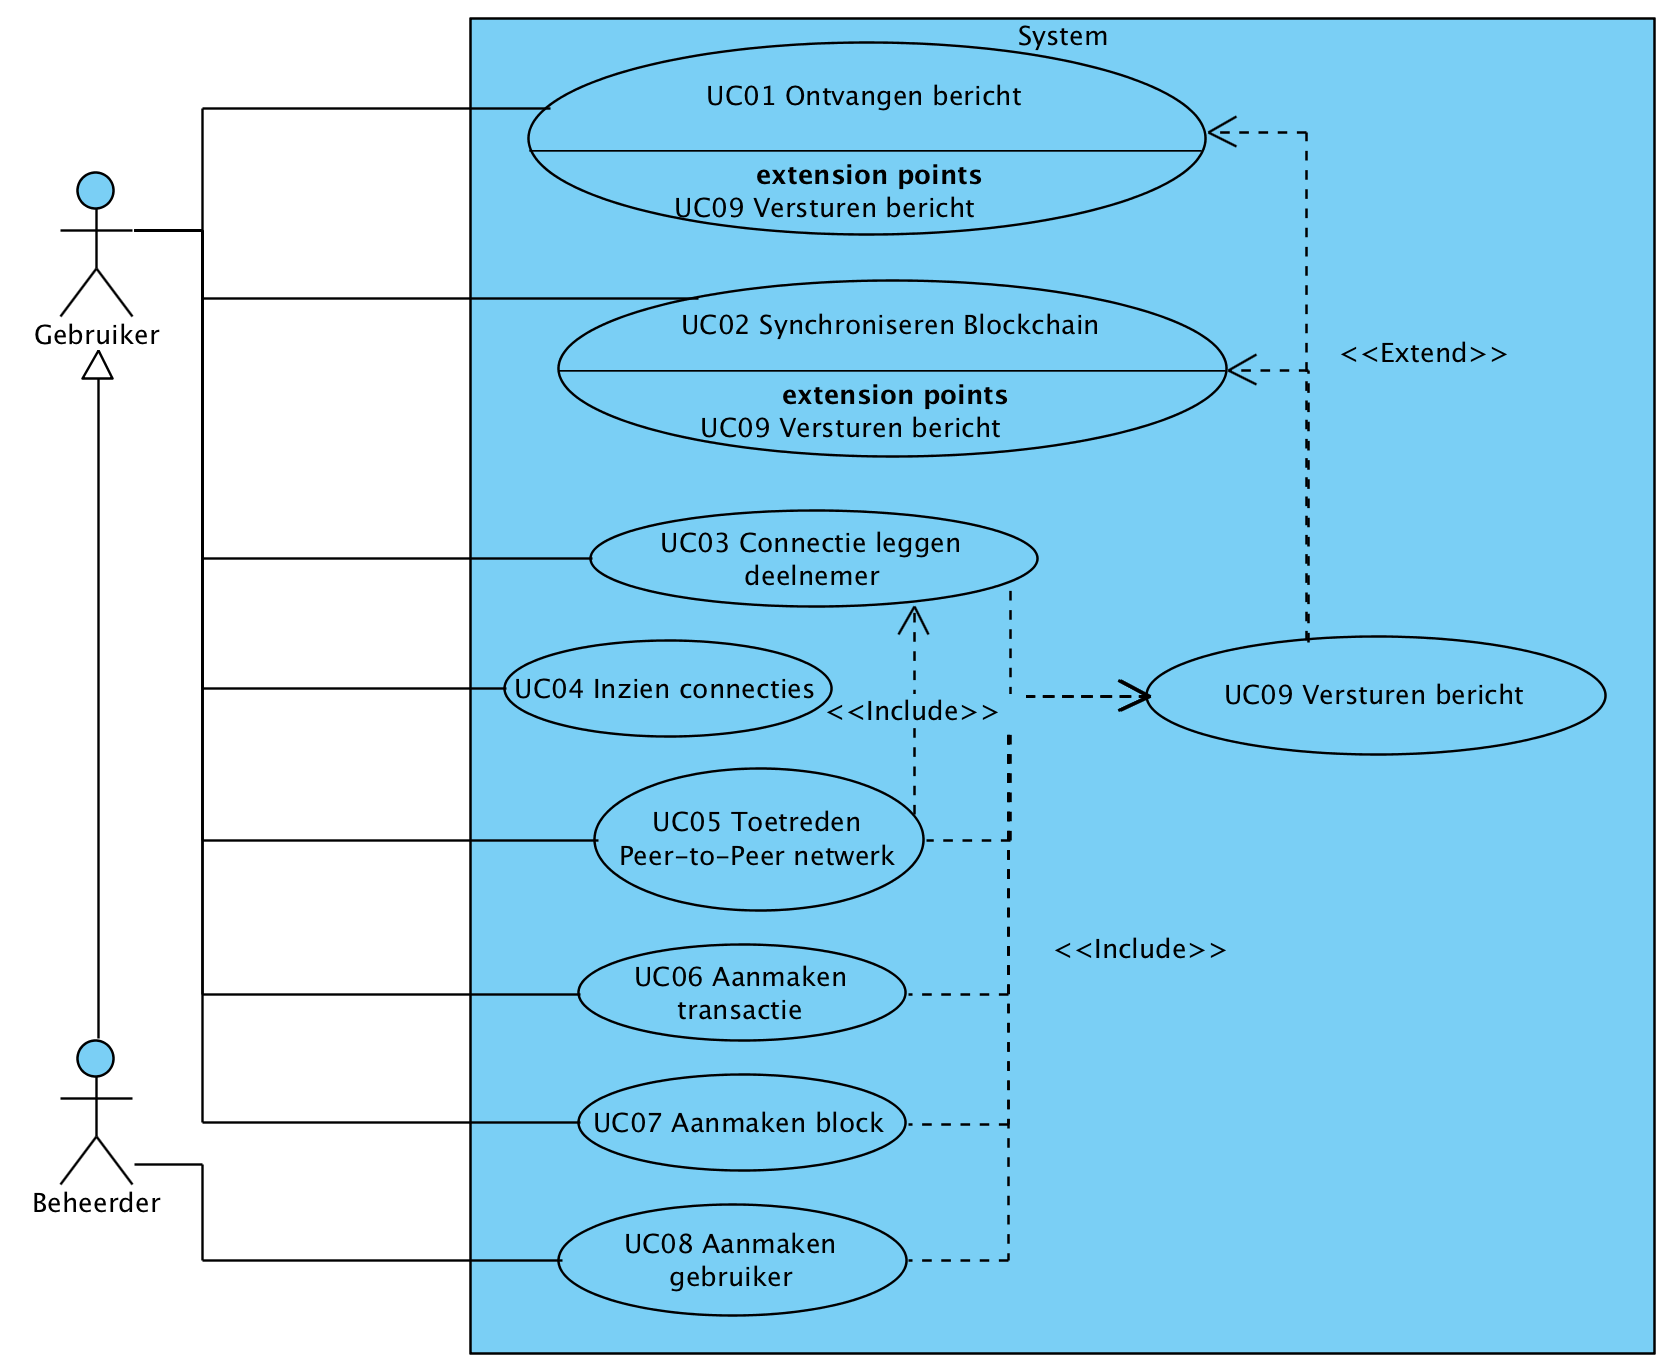
\includegraphics[width=1\textwidth]{use_case_diagram}
  \caption[Use-case Diagram] {
    Use-case diagram waarin de rollen binnen het systeem te zien zijn en de acties die zij kunnen uitvoeren.
  }
\end{figure}

% Sets subnumbering instead of letters
\renewcommand{\labelenumii}{\theenumii}
\renewcommand{\theenumii}{\theenumi.\arabic{enumii}.}

\begin{usecase}{Ontvangen bericht}
  \addrow{Id}{UC01}
  \addrow{Requirements}{FR03, FR02, FR01}
  \addrow{Beschrijving}{Gebruiker ontvangt een bericht van een deelnemer uit het Peer-to-Peer netwerk}
  \addrow{Primaire actor}{Gebruiker}
  \addrow{Secundaire actor}{-}
  \addrow{Precondition}{De gebruiker is verbonden met het Peer-to-Peer netwerk}
  \addmulrow{Main flow}{
    \item Systeem ontvangt bericht
    \item Systeem valideert bericht type
    \item Systeem deserialiseert bericht
    \item Systeem controleert of er antwoord verstuurd dient te worden
    \item Use-case eindigt (Postconditie: Success1)
  }
  \addrow{Postconditie}{
    Success1: Systeem heeft een bericht verstuurd naar verzender
    Failure1: Systeem is ongewijzigd
  }
  \addmulrow{Alternatieve flows}{
    \item Bericht is van type \textit{req} (na MF4)
    \begin{enumerate}
      \item Systeem valideert dat gevraagde data aanwezig is
      \item Systeem creërt \textit{data} bericht
      \item Systeem voert \textit{UC09 - Versturen bericht} uit
      \item Use-case eindigt (Postconditie: Success1)
    \end{enumerate}
    \item Bericht is van type \textit{inv} (na MF4)
    \begin{enumerate}
      \item Systeem valideert dat aangeboden data niet aanwezig is
      \item Systeem creërt \textit{req} bericht
      \item Systeem voert \textit{UC09 - Versturen bericht} uit
      \item Use-case eindigt (Postconditie: Success1) 
    \end{enumerate} 
  }
\end{usecase}

\begin{usecase}{Synchroniseren Blockchain}
  \addrow{Id}{UC02}
  \addrow{Requirements}{FR02}
  \addrow{Beschrijving}{Gebruiker haalt Blockchain informatie op van een verbonden deelnemer}
  \addrow{Primaire actor}{Gebruiker}
  \addrow{Secundaire actor}{-}
  \addrow{Precondition}{De gebruiker is verbonden met het Peer-to-Peer netwerk}
  \addmulrow{Main flow}{
    \item Systeem maakt \textit{req} bericht
    \item Systeem voert \textit{UC09 - Versturen bericht} uit
    \item Systeem voert \textit{UC01 - Ontvangen bericht} uit
    \item Systeem hercreëert Blockchain van ontvangen data
    \item Use case eindigt (Postconditie: Success1)
  }
  \addrow{Postconditie}{
    Success1: Gebruiker is up-to-date met de laatste Blockchain data
  }
\end{usecase}

\begin{usecase}{Connectie leggen deelnemer}
  \addrow{Id}{UC03}
  \addrow{Requirements}{FR03}
  \addrow{Beschrijving}{Gebruiker maakt connectie met een deelnemer uit het Peer-to-Peer netwerk}
  \addrow{Primaire actor}{Gebruiker}
  \addrow{Secundaire actor}{-}
  \addrow{Precondition}{De gebruiker is verbonden met het Peer-to-Peer netwerk}
  \addmulrow{Main flow}{
    \item Systeem vraagt om adresgegevens(ip, poort) van deelnemer
    \item Actor vult informatie in
    \item Systeem valideert adresgegevens
    \item Systeem valideert dat deelnemer bereikbaar is
    \item Systeem creërt \textit{auth} bericht
    \item Systeem voert \textit{UC09 - Versturen bericht} uit
    \item Use-case eindigt (Postconditie: Succes1)
  }
  \addrow{Postconditie}{
    Succes1: De gebruiker is verbonden met de deelnemer
    Failure1: Systeem is ongewijzigd
  }
  \addmulrow{Alternatieve flow} {
    \item Invalide adresgegevens (na MF3)
    \begin{enumerate}
      \item Use-case gaat verder bij MF1
    \end{enumerate}
    \item Deelnemer is niet bereikbaar (na MF4)
    \begin{enumerate}
      \item Systeem toont foutmelding
      \item Use-case eindigt (Postconditie: Failure1)
    \end{enumerate}
    \item Actor annuleert (Overal)
  }
\end{usecase}

\begin{usecase}{Toetreden Peer-to-Peer netwerk}
  \addrow{Id}{UC05}
  \addrow{Requirements}{FR05}
  \addrow{Beschrijving}{Gebruiker wilt deel uitmaken van het Peer-to-Peer netwerk}
  \addrow{Primaire actor}{Gebruiker}
  \addrow{Secundaire actor}{-}
  \addrow{Precondition}{Actor heeft een account tot zijn beschikking}
  \addmulrow{Main flow}{
    \item Actor start systeem
    \item Systeem controleert of de actor niet reeds connectie heeft gemaakt
    \item Systeem zoekt bootstrap node op
    \item Systeem verstuurd authenticatie bericht naar bootstrap node
    \item Systeem voert \textit{UC01 - Ontvangen bericht} uit
    \item Systeem ontvangt lijst van andere deelnemers die verbinding gemaakt hebben met het netwerk
    \item Systeem voert \textit{UC03 - Connectie leggen deelnemer} uit
    \item Systeem voert \textit{UC01 - Ontvangen bericht} uit 
    \item Systeem slaat adresgegevens (ip, port) op van deelnemer
    \item Systeem voert \textit{UC02 - Synchroniseren Blockchain} uit
    \item Use-case eindigt (Postconditie: Success1)
  }
  \addrow{Post conditie}{
    Success1: Actor is actief in het netwerk.
    Failure1: Systeem is ongewijzigd
  }
  \addmulrow{Alternatieve flows}{
    \item AF1: Gebruiker heeft reeds connectie gemaakt (na MF2)
    \begin{enumerate}
    \item Systeem haalt lijst van opgeslagen deelnemers op
    \item Systeem probeert verbinding te maken met deelnemers
    \item Systeem voert \textit{UC01 - Ontvangen bericht} uit
    \item Use-case eindigt (Postconditie: Success1)
    \end{enumerate}

    \item AF2: Actor gebruikt verkeerde identificatie (na MF5)
    \begin{enumerate}
      \item Systeem toont foutmelding
      \item Use-case eindigt (Postconditie: Failure1)
    \end{enumerate}
  }
\end{usecase}

\begin{usecase}{Aanmaken transactie}
  \addrow{Id}{UC06}
  \addrow{Requirements}{FR01}
  \addrow{Beschrijving}{Gebruiker wilt een transactie opslaan in de Blockchain}
  \addrow{Primaire actor}{Gebruiker}
  \addrow{Secundaire actor}{-}
  \addrow{Precondition}{De gebruiker is verbonden met het Peer-to-Peer netwerk}
  \addmulrow{Main flow}{
    \item Systeem vraagt om public key ontvanger
    \item Actor vult public key in
    \item Systeem valideert public key
    \item Systeem vraagt om type transactie
    \item Actor selecteert type transactie
    \item Systeem vraag aanvullende informatie gebaseerd op geselecteerde type
    \item Actor vult aanvullende informatie in
    \item Systeem valideert aanvullende informatie
    \item Systeem maakt transactie van geselecteerde transactietype aan
    \item Systeem creërt een \textit{inv} bericht
    \item Systeem voert \textit{UC09 - Versturen bericht} uit
    \item Use-case eindigt (Postconditie: Success1)
  }
  \addrow{Post conditie}{
    Success1: Systeem heeft een transactie aangemaakt
  }
  \addmulrow{Alternatieve flows}{
    \item Actor annuleert (Overal)
  }
\end{usecase}

\begin{usecase}{Versturen bericht}
  \addrow{Id}{UC09}
  \addrow{Requirements}{FR01}
  \addrow{Beschrijving}{Gebruiker verstuurd bericht over het netwerk}
  \addrow{Primaire actor}{Gebruiker}
  \addrow{Secundaire actor}{-}
  \addrow{Precondition}{De gebruiker is verbonden met het Peer-to-Peer netwerk}
  \addmulrow{Main flow}{
    \item Systeem controleert bericht type
    \item Systeem verstuurd bericht naar deelnemer
    \item Use-case eindigt (Postconditie: Success1)
  }
  \addrow{Postconditie}{
    Success1: Systeem heeft bericht verstuurd naar deelnemer
    Success2: Systeem heeft bericht verstuurd naar alle verbonden deelnemers
  }
  \addmulrow{Alternatieve flows} {
    \item Bericht is van type \textit{inv} (na MF1)
    \begin{enumerate}
      \item Systeem haalt lijst van alle verbonden deelnemers op
      \item Systeem verstuurd bericht naar alle verbonden deelnemers
      \item Use-case eindigt (Postconditie: Success2)
    \end{enumerate}
  }
\end{usecase}
\newpage